\documentclass[journal, a4paper]{IEEEtran}

% some very useful LaTeX packages include:

%\usepackage{cite}      % Written by Donald Arseneau
                        % V1.6 and later of IEEEtran pre-defines the format
                        % of the cite.sty package \cite{} output to follow
                        % that of IEEE. Loading the cite package will
                        % result in citation numbers being automatically
                        % sorted and properly "ranged". i.e.,
                        % [1], [9], [2], [7], [5], [6]
                        % (without using cite.sty)
                        % will become:
                        % [1], [2], [5]--[7], [9] (using cite.sty)
                        % cite.sty's \cite will automatically add leading
                        % space, if needed. Use cite.sty's noadjust option
                        % (cite.sty V3.8 and later) if you want to turn this
                        % off. cite.sty is already installed on most LaTeX
                        % systems. The latest version can be obtained at:
                        % http://www.ctan.org/tex-archive/macros/latex/contrib/supported/cite/
\usepackage{amsfonts}
\usepackage{graphicx}   % Written by David Carlisle and Sebastian Rahtz
                        % Required if you want graphics, photos, etc.
                        % graphicx.sty is already installed on most LaTeX
                        % systems. The latest version and documentation can
                        % be obtained at:
                        % http://www.ctan.org/tex-archive/macros/latex/required/graphics/
                        % Another good source of documentation is "Using
                        % Imported Graphics in LaTeX2e" by Keith Reckdahl
                        % which can be found as esplatex.ps and epslatex.pdf
                        % at: http://www.ctan.org/tex-archive/info/

%\usepackage{psfrag}    % Written by Craig Barratt, Michael C. Grant,
                        % and David Carlisle
                        % This package allows you to substitute LaTeX
                        % commands for text in imported EPS graphic files.
                        % In this way, LaTeX symbols can be placed into
                        % graphics that have been generated by other
                        % applications. You must use latex->dvips->ps2pdf
                        % workflow (not direct pdf output from pdflatex) if
                        % you wish to use this capability because it works
                        % via some PostScript tricks. Alternatively, the
                        % graphics could be processed as separate files via
                        % psfrag and dvips, then converted to PDF for
                        % inclusion in the main file which uses pdflatex.
                        % Docs are in "The PSfrag System" by Michael C. Grant
                        % and David Carlisle. There is also some information
                        % about using psfrag in "Using Imported Graphics in
                        % LaTeX2e" by Keith Reckdahl which documents the
                        % graphicx package (see above). The psfrag package
                        % and documentation can be obtained at:
                        % http://www.ctan.org/tex-archive/macros/latex/contrib/supported/psfrag/

%\usepackage{subfigure} % Written by Steven Douglas Cochran
                        % This package makes it easy to put subfigures
                        % in your figures. i.e., "figure 1a and 1b"
                        % Docs are in "Using Imported Graphics in LaTeX2e"
                        % by Keith Reckdahl which also documents the graphicx
                        % package (see above). subfigure.sty is already
                        % installed on most LaTeX systems. The latest version
                        % and documentation can be obtained at:
                        % http://www.ctan.org/tex-archive/macros/latex/contrib/supported/subfigure/

\usepackage{url}        % Written by Donald Arseneau
                        % Provides better support for handling and breaking
                        % URLs. url.sty is already installed on most LaTeX
                        % systems. The latest version can be obtained at:
                        % http://www.ctan.org/tex-archive/macros/latex/contrib/other/misc/
                        % Read the url.sty source comments for usage information.

%\usepackage{stfloats}  % Written by Sigitas Tolusis
                        % Gives LaTeX2e the ability to do double column
                        % floats at the bottom of the page as well as the top.
                        % (e.g., "\begin{figure*}[!b]" is not normally
                        % possible in LaTeX2e). This is an invasive package
                        % which rewrites many portions of the LaTeX2e output
                        % routines. It may not work with other packages that
                        % modify the LaTeX2e output routine and/or with other
                        % versions of LaTeX. The latest version and
                        % documentation can be obtained at:
                        % http://www.ctan.org/tex-archive/macros/latex/contrib/supported/sttools/
                        % Documentation is contained in the stfloats.sty
                        % comments as well as in the presfull.pdf file.
                        % Do not use the stfloats baselinefloat ability as
                        % IEEE does not allow \baselineskip to stretch.
                        % Authors submitting work to the IEEE should note
                        % that IEEE rarely uses double column equations and
                        % that authors should try to avoid such use.
                        % Do not be tempted to use the cuted.sty or
                        % midfloat.sty package (by the same author) as IEEE
                        % does not format its papers in such ways.

\usepackage{amsmath}    % From the American Mathematical Society
                        % A popular package that provides many helpful commands
                        % for dealing with mathematics. Note that the AMSmath
                        % package sets \interdisplaylinepenalty to 10000 thus
                        % preventing page breaks from occurring within multiline
                        % equations. Use:
%\interdisplaylinepenalty=2500
                        % after loading amsmath to restore such page breaks
                        % as IEEEtran.cls normally does. amsmath.sty is already
                        % installed on most LaTeX systems. The latest version
                        % and documentation can be obtained at:
                        % http://www.ctan.org/tex-archive/macros/latex/required/amslatex/math/



% Other popular packages for formatting tables and equations include:

%\usepackage{array}
% Frank Mittelbach's and David Carlisle's array.sty which improves the
% LaTeX2e array and tabular environments to provide better appearances and
% additional user controls. array.sty is already installed on most systems.
% The latest version and documentation can be obtained at:
% http://www.ctan.org/tex-archive/macros/latex/required/tools/

% V1.6 of IEEEtran contains the IEEEeqnarray family of commands that can
% be used to generate multiline equations as well as matrices, tables, etc.

% Also of notable interest:
% Scott Pakin's eqparbox package for creating (automatically sized) equal
% width boxes. Available:
% http://www.ctan.org/tex-archive/macros/latex/contrib/supported/eqparbox/

% *** Do not adjust lengths that control margins, column widths, etc. ***
% *** Do not use packages that alter fonts (such as pslatex).         ***
% There should be no need to do such things with IEEEtran.cls V1.6 and later.


% Your document starts here!
\begin{document}
\begin{titlepage}

\newcommand{\HRule}{\rule{\linewidth}{0.5mm}} % Defines a new command for the horizontal lines, change thickness here

\center % Center everything on the page
 %----------------------------------------------------------------------------------------
%	LOGO SECTION
%----------------------------------------------------------------------------------------

~\\[1cm]

\includegraphics{SCUT.png}\\[2cm] % Include a department/university logo - this will require the graphicx package

%----------------------------------------------------------------------------------------
%	TITLE SECTION
%----------------------------------------------------------------------------------------

\HRule \\[1cm]
{ \huge \bfseries The Experiment Report of \textit{Machine Learning} }\\[0.6cm] % Title of your document
\HRule \\[2cm]
%----------------------------------------------------------------------------------------
%	HEADING SECTIONS
%----------------------------------------------------------------------------------------


\textsc{\LARGE \textbf{School:} School of Software Engineering}\\[1cm]
\textsc{\LARGE \textbf{Subject:} Software Engineering}\\[2cm] 

 
%----------------------------------------------------------------------------------------
%	AUTHOR SECTION
%----------------------------------------------------------------------------------------

\begin{minipage}{0.4\textwidth}
\begin{flushleft} \large
\emph{Author:}\\
Panan Wu % Your name
\end{flushleft}
\end{minipage}
~
\begin{minipage}{0.4\textwidth}
\begin{flushright} \large
\emph{Supervisor:} \\
Mingkui Tan % Supervisor's Name
\end{flushright}
\end{minipage}\\[2cm]
~
\begin{minipage}{0.4\textwidth}
\begin{flushleft} \large
\emph{Student ID:}\\
201630665908
\end{flushleft}
\end{minipage}
~
\begin{minipage}{0.4\textwidth}
\begin{flushright} \large
\emph{Grade:} \\
Undergraduate
\end{flushright}
\end{minipage}\\[2cm]

% If you don't want a supervisor, uncomment the two lines below and remove the section above
%\Large \emph{Author:}\\
%John \textsc{Smith}\\[3cm] % Your name

%----------------------------------------------------------------------------------------
%	DATE SECTION
%----------------------------------------------------------------------------------------

{\large \today}\\[2cm] % Date, change the \today to a set date if you want to be precise

 
%----------------------------------------------------------------------------------------

\vfill % Fill the rest of the page with whitespace

\end{titlepage}

% Define document title and author
	\title{Linear Regression and Stochastic Gradient Descent}
	\maketitle

% Write abstract here
\begin{abstract}
In this experiment, I conduct a linear regressor and update parameters with stochastic gradient descent and closed-form solution using scaled Housing dataset in LIBSVM Data. I evaluated the two methods mentioned above by plotting the loss value and root mean square error (rmse) during the parameters update process. The experiment result shows that the process of parameters updates with closed-form solution is stable and parameters reach the optimal solution within one iteration, and parameters update with stochastic gradient descent needs multiple iterations to reach a good solution and unstable.

\end{abstract}

% Each section begins with a \section{title} command
\section{Introduction}
	% \PARstart{}{} creates a tall first letter for this first paragraph
\PARstart{L}{inear} regression is a classical way to solve regression problems. We have mutiple ways to update parameters like closed-form solution and stochastic gradient descent. Closed-form solution is very accurate but time consuming while stochastic gradient descent is efficient but not so accurate. 

In this experiment, I implement two versions of linear regression: one with closed-form solution and another with stochastic gradient descent. By plotting the loss in training, we can intuitively know how these two methods update parameters.

The motivations of this experiment are: (1) further understand of linear regression, closed-form solution and Stochastic gradient descent, (2) conduct some experiments under small scale dataset and (3) realize the process of optimization and adjusting parameters.

% Main Part
\section{Methods and Theory}
\subsection{Linear Regression}
Linear regression describes the linear relationship between a predictor variable and a response variable.

The input of linear regression $\textbf{X}$ is within the input space $\mathbb{R}^m$ (m is corresponding to the number of features), and it's also called feature, covariants, predictors, etc.
The groundtruth of linear regression $\textbf{Y}$ is the value that we use $X$ to predict.
And the goal of linear regression is to learn a hypothesis or model $f : \textbf{X} \rightarrow \textbf{Y}$.

In order to learn a model, we first need to construct a dataset. Given set of input, output pairs: \begin{equation}
D=\{(x_i, y_i)\}^{n}_{i=1}
\end{equation} In the equation mentioned above, $x_i $ is a single sample of input, $y_i$ is a groundtruth of this sample and n is the number of training samples. To learn the best model on dataset $D$, we use parameters \textbf{w} to help us make predict. And the model funtion is:
\begin{equation}
\begin{split}
\begin{aligned}
f(\textbf{x}; w_0; \textbf{w}) &= w_0 + w_1x_1 + ... + w_mx_m \\
&= \sum_{j=1}^{n}{w_jx_j}+w_0 \\
&= \textbf{w}^T\textbf{x} + w_0
\end{aligned}
\end{split}
\end{equation}
To evaluate and update our model, we need to define the difference between our predict and the groundtruth. We use loss function \textbf{Least squared loss} to measure the difference. 
\begin{equation}
\begin{split}
\begin{aligned}
\mathcal{L}_D(\textbf{w})&= \frac{1}{2}\sum_{i=1}^{n}{(y_i-f(\textbf{x}_i; \textbf{w}))}^2 \\
&= \frac{1}{2}\sum_{i=1}^{n}{(y_i-\hat{y_i})}^2 \\
\end{aligned}
\end{split}
\end{equation}
And our goal is to find \textbf{w*} that minimizes loss $\mathcal{L}$.
\begin{equation}
\textbf{w}^* = \mathop{\arg\min}_{\textbf{w}} \mathcal{L}_D(\textbf{w})
\end{equation}
\subsection{Closed-form Solution}
To calculate the gradient of loss function, we first need to represent the loss function as a function in matrix form: 
\begin{equation}
\begin{split}
\begin{aligned}
\mathcal{L}_D(\textbf{w})&= \frac{1}{2}\sum_{i=1}^{n}{(y_i-f(\textbf{x}_i; \textbf{w}))}^2 \\
&= \frac{1}{2}(\textbf{y}-\textbf{Xw})^T(\textbf{y}-\textbf{Xw})) \\
&= \frac{1}{2}(\textbf{y}^T\textbf{y}-2\textbf{w}^T\textbf{X}^T\textbf{y}+\textbf{w}^T\textbf{X}^T\textbf{Xw} ) \\
\end{aligned}
\end{split}
\end{equation}
And then we calculate the partial derivative of the loss function for the parameter \textbf{w}:
\begin{equation}
\begin{split}
\begin{aligned}
\frac{\partial\mathcal{L}_D(\textbf{w})}{\partial\textbf{w}}
&= \frac{1}{2}(\frac{\partial\textbf{y}^T\textbf{y}}{\partial\textbf{w}}-\frac{\partial2\textbf{w}^T\textbf{X}^T\textbf{y}}{\partial\textbf{w}}+\frac{\partial\textbf{w}^T\textbf{X}^T\textbf{Xw}}{\partial\textbf{w}} ) \\
&= \frac{1}{2}(-2\textbf{X}^T\textbf{y}+(\textbf{X}^T\textbf{X}+(\textbf{X}^T\textbf{X})^T)\textbf{w}) \\
&= -\textbf{X}^T\textbf{y} + \textbf{X}^T\textbf{X}\textbf{w}
\end{aligned}
\end{split}
\end{equation}

To get analytical solution, we make the partial derivative equals to zero and calculate the value of parameter w:

\begin{equation}
\begin{split}
\begin{aligned}
\label{equ:7}
\frac{\partial\mathcal{L}_D(\textbf{w})}{\partial\textbf{w}}
&= -\textbf{X}^T\textbf{y} + \textbf{X}^T\textbf{X}\textbf{w} = 0 \\
&\Rightarrow\textbf{w} = (\textbf{X}^T\textbf{X})^{-1}\textbf{X}^T\textbf{y}
\end{aligned}
\end{split}
\end{equation}

As we have seen in the equation, we have to calculate the inverse matrix of $\textbf{X}^T\textbf{X}$, which is not only time consuming but impossible for most matrices. Thus most of the time, we will use gradient descent to update our parameters, while stochastic gradient descent is a typical variant of gradient descent.

\subsection{Gradient Descent}
In the gradient descent, I minimize loss by repeated gradient steps(when no closed form). First, I  compute gradient of loss with respect to parameters : $\frac{\partial\mathcal{L}_D(\textbf{w})}{\partial\textbf{w}}$. Then I update parameters with rate $\eta$ which is called learning rate.

\begin{equation}
\textbf{w}^\prime \rightarrow \textbf{w} - \eta\frac{\partial\mathcal{L}_D(\textbf{w})}{\partial\textbf{w}}
\end{equation}

\subsection{Stochastic Gradient Descent}
The main idea of stochastic gradient descent (SGD) are to estimate function and gradient from a small, current subsample of training data and with enough iterations and data, loss function will converge to the true minimum.
In SDG the true gradient of $\mathcal{L}(w)$ is approximated by agradient of a single example:
\begin{equation}
\textbf{w} := \textbf{w} - \eta\nabla\mathcal{L}_i(\textbf{w})
\end{equation}
Although random noise is introduced, it behaves like gradient descent in its expectation.
\section{Experiments}
\subsection{Dataset}

The dataset I used in this experiment is scaled Housing dataset from LIBSVM Data. There are 506 instances and 13 features in this dataset. The data had been scaled into [-1,1] for better prediction. What we need to do is to predict the house price according to its features like averge number of rooms per dwelling. Because they don't divide the training set and test set, we need to divide the training set and test set by ourselves.

\subsection{Implementation}

\subsubsection{Closed-form Solution}
.

First of all, I load the Housing dataset using $load\_svmlight\_file$ function in sklearn library. Then, I divide dataset into training set and validation set using $train\_test\_split$ function. I set the test size to 0.25.

When it comes to initialize parameters. I choose to set all parameter into zero, initialize it randomly and with normal distribution separately to determine which one is the best.After that, I calculate the closed-form solution by equation \ref{equ:7} and update parameters. And then I calculate loss of both training set and validation set. I repeat this process 300 times and output the loss during each process.

Finally, I plot both training loss and validation loss during parameter update. As we can see from Fig.\ref{fig:closed0}, the closed-form solution finds the best parameters at the first iteration, the loss of training set and validation set are stable. And then I plot the validation rmse variation with the number of iterations, the rmse of valiadation is still stable. Finally, I output and plot the mean loss with different parameter initializers, as shown in TABLE~\ref{tab:lossInitial} and Fig.~\ref{fig:closed2}, the initializer in closed-form solution doesn't affect the loss function at all.

	\begin{figure}[!hbt]
		\begin{center}
		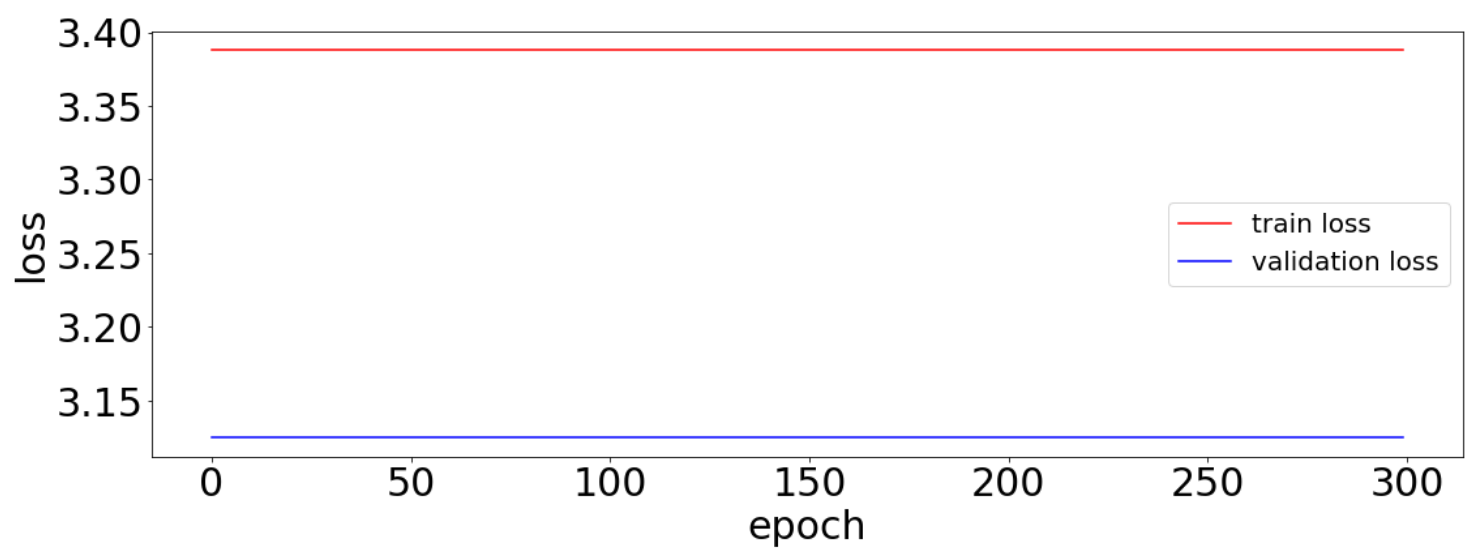
\includegraphics[width=\columnwidth]{closed-form0}
		\caption{The loss varing with the number of iterations.}
		\label{fig:closed0}
		\end{center}
	\end{figure}
	
	\begin{figure}[!hbt]
		\begin{center}
		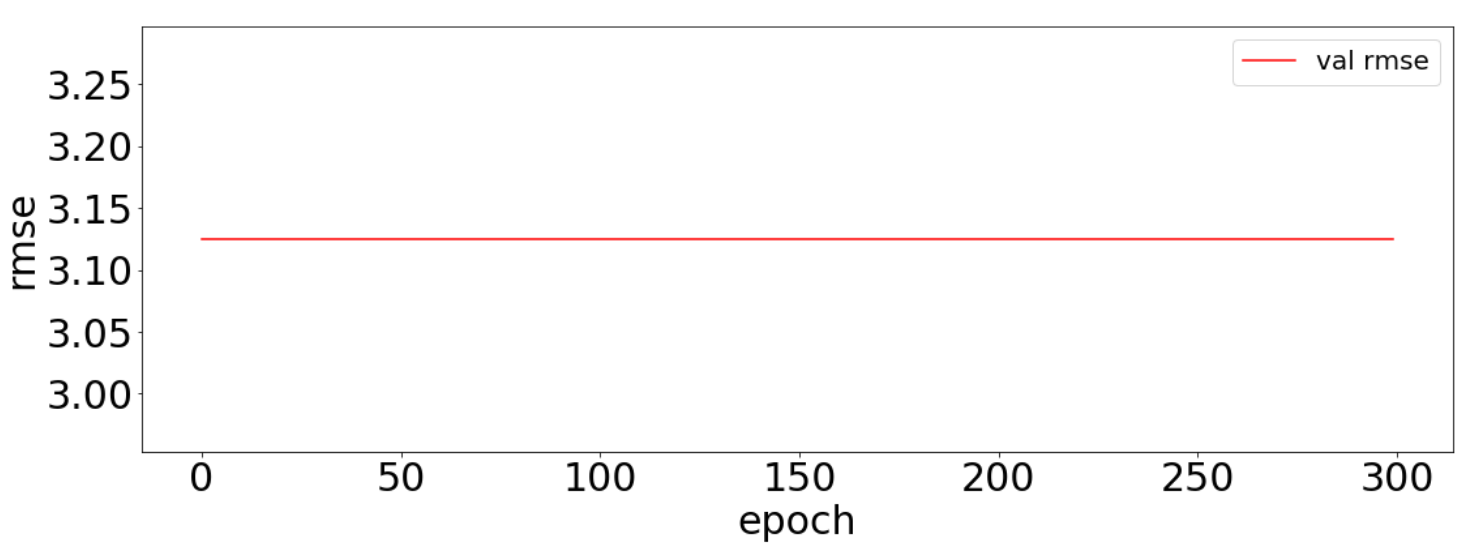
\includegraphics[width=\columnwidth]{closed-form1}
		\caption{The rmse varing with the number of iterations.}
		\label{fig:closed1}
		\end{center}
	\end{figure}

	\begin{table}[!hbt]
		\begin{center}
		\caption{Mean loss with different initializer}
		\label{tab:lossInitial}
		\begin{tabular}{|c|c|}
			\hline
			Initializer & Mean Loss \\
			\hline
			Zero Initializer & 3.394 \\
			\hline
			Random Initializer & 3.394 \\
			\hline
			Normal Initializer & 3.394 \\
			\hline
		\end{tabular}
		\end{center}
	\end{table}

	\begin{figure}[!hbt]
		\begin{center}
		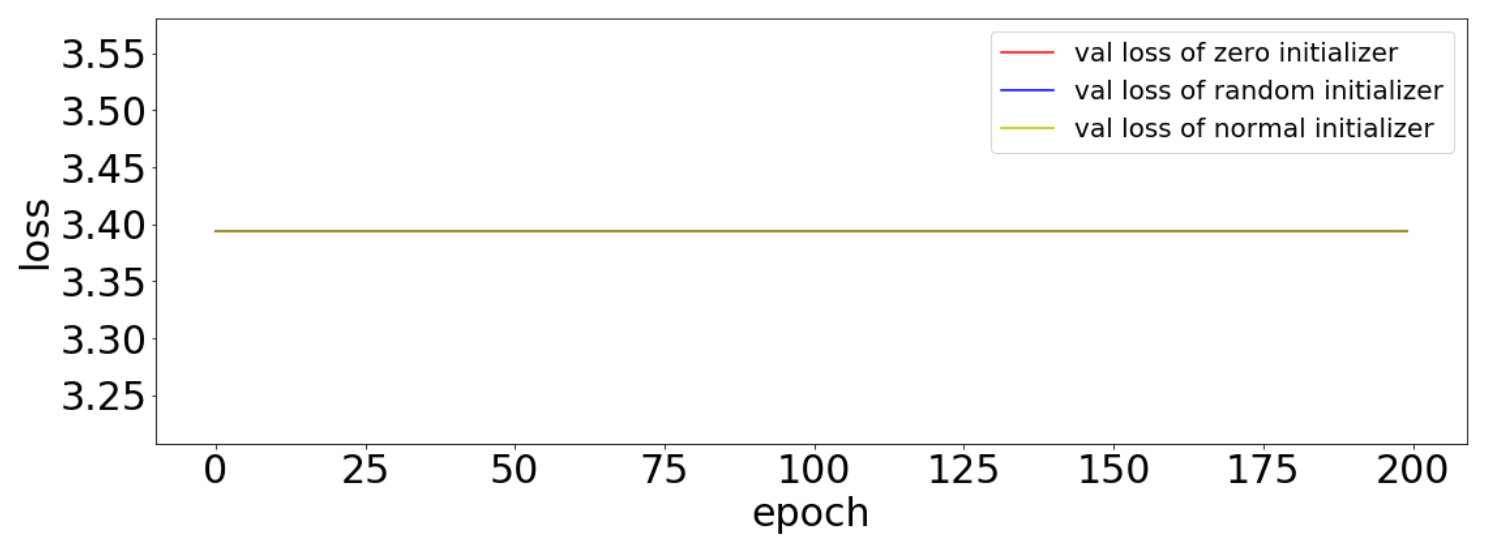
\includegraphics[width=\columnwidth]{closed-form2}
		\caption{The loss varing with the number of iterations and different intializers.}
		\label{fig:closed2}
		\end{center}
	\end{figure}
	


\subsubsection{Stochatic Gradient Descent}
.

As the same in closed-form solution experiment, I read training data and split it into two parts. During training, I set learning rate to 0.001 and max epoch to 300. I still try three types of parameter initializers. When it comes to parameters update, I first randomly choose a sample from training set and update parameters according to its partial derivative, and I calculate and store the training loss and validation loss with parameters just update.

As shown in Fig.~\ref{fig:sgd0}, the training loss is unstable, but the validation loss and rmse are stable decline. Different initializers bring different loss mean values, which means that choosing different initializers in sgd will have a certain impact on the results, and zero intializer seems better than other two initializers in this dataset.

	\begin{figure}[!hbt]
		\begin{center}
		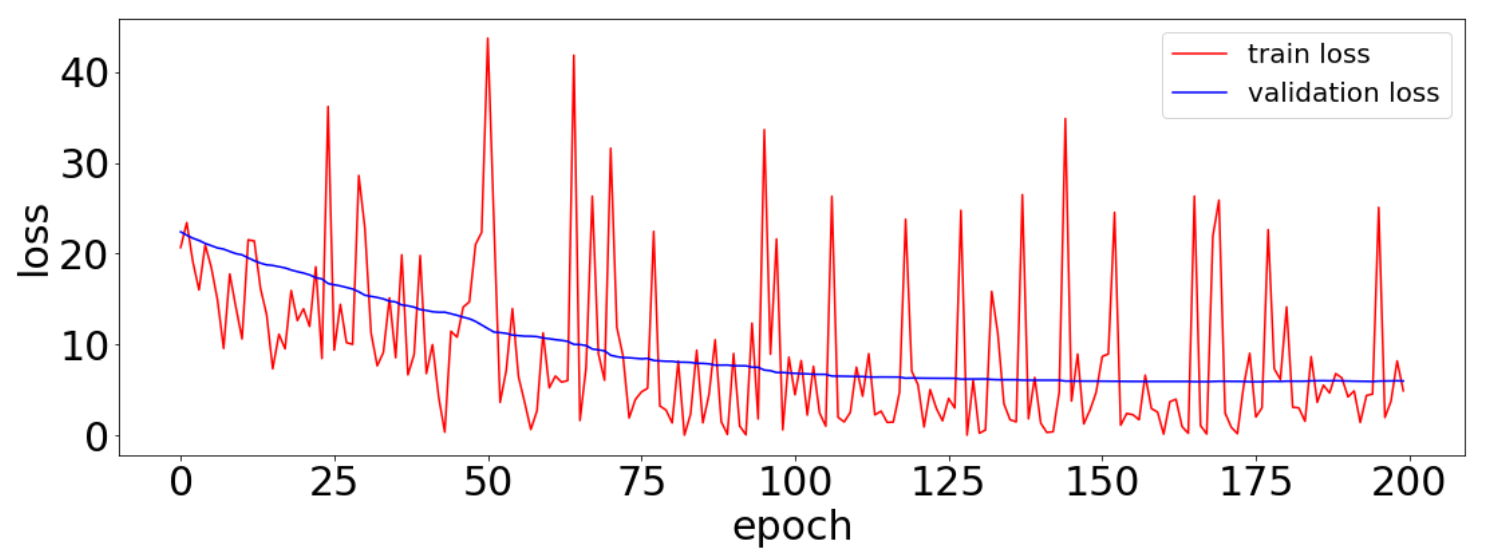
\includegraphics[width=\columnwidth]{sgd0}
		\caption{The loss varing with the number of iterations.}
		\label{fig:sgd0}
		\end{center}
	\end{figure}
	
	\begin{figure}[!hbt]
		\begin{center}
		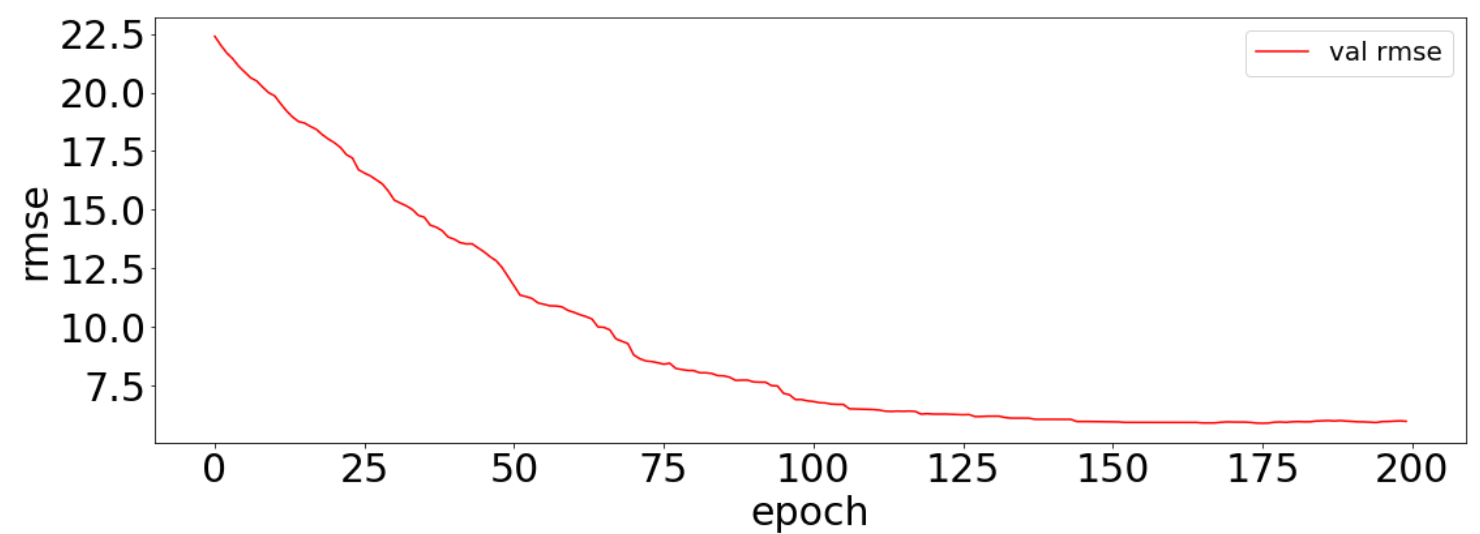
\includegraphics[width=\columnwidth]{sgd1}
		\caption{The rmse varing with the number of iterations.}
		\label{fig:sgd1}
		\end{center}
	\end{figure}

	\begin{table}[!hbt]
		\begin{center}
		\caption{Mean loss with different initializer}
		\label{tab:lossInitial1}
		\begin{tabular}{|c|c|}
			\hline
			Initializer & Mean Loss \\
			\hline
			Zero Initializer & 10.123 \\
			\hline
			Random Initializer & 10.553 \\
			\hline
			Normal Initializer & 11.342 \\
			\hline
		\end{tabular}
		\end{center}
	\end{table}

	\begin{figure}[!hbt]
		\begin{center}
		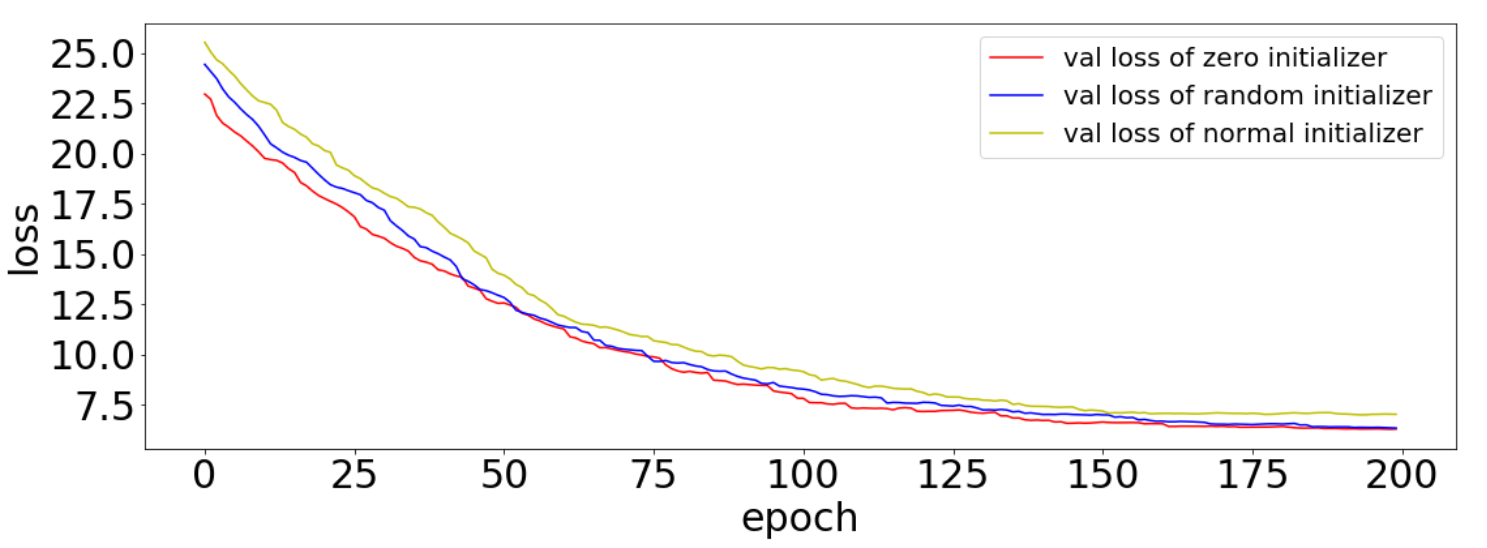
\includegraphics[width=\columnwidth]{sgd2}
		\caption{The loss varing with the number of iterations and different intializers.}
		\label{fig:sgd2}
		\end{center}
	\end{figure}
	
Finally, I compared the result of two methods mentioned above. We can know from Table~\ref{tab:loss} that closed-form solution has lower  validation loss than sgd. The final training loss of sgd is lower than that of closed form. This result means that sgd may be better than closed form. After all, it contains many random factors in training process, but it has two more hyper-parameters that need to be artificially adjusted.

	\begin{table}[!hbt]
		\begin{center}
		\caption{Mean loss with different initializer}
		\label{tab:loss}
		\begin{tabular}{|c|c|c|}
			\hline
			Metrics & Closed-form & Sgd \\
			\hline
			Final training loss & 3.3876407032391738 & 3.068910779095976 \\
			\hline
			Final validation loss & 3.1251863328930667 & 5.648078628287903\\
			\hline
		\end{tabular}
		\end{center}
	\end{table}

\section{Conclusion}

In this experiment, I implement linear regression and update parameters with closed-form solution and stochastic gradient descent, and I make comparison between the two update methods mentioned above. From what has been shown above, we may safely draw the conclusion that the closed-form solution is accurate and doesn't need iterations to update, while the sgd needs several iterations to reach a good solution. But we need to try other kinds of dataset to evalute these two methods better.

During this experiment, I realized what I learned in class, which enhanced my code practice ability. By comparing these two methods and writing experimental reports, I came into contact with a little scientific research. And it has increased my knowledge.

% Your document ends here!
\end{document}